\documentclass{article}
\usepackage[margin=0.5in]{geometry} % Set margins to 0.5"
\geometry{top=0.5in}
\usepackage{amsmath}
\usepackage{graphicx}
\usepackage{hyperref}
% chktex-file 1
\title{Final Project Update: \\ Betting on the Cardinal as a Markov Decision Process}
\author{Zain Jamal & Sean Auer}
\date{\today}
\begin{document}
\maketitle

\section*{Problem Statement}

The primary objective of this project is to formulate a Markov Decision Process (MDP) validated by the betting outcomes for Stanford's 2023 football season. 
We aim to model the decision-making process of a bettor making a moneyline bet on Stanford sequentially each week of the regular season of college football,
using available statistics and publically released betting metrics as the basis for developing a realistic rewards model and eventually determining an optimum policy.

\section*{Data Acquisition and Preprocessing}

The first step in the project was to acquire relevant data from publically available statistics and sportsbooks websites, such as \texttt{collegefootballdata.com} on Stanford’s 2023 football season. 
After examining available datasets regarding team and individual performance, strength of schedule metrics, and odds from various sportsbooks, it was decided to focus on four key datasets: 
\begin{itemize}
    \item Betting data - Moneyline and spread numbers available at time of kickoff
    \item Advanced metrics - Success Rates (SR), Expected Points Added (EPA)
    \item Generalzed statistics from prior weeks - Final scores, power rating metrics
    \item Team statistics - Team totals for turnovers, yardage, and points
\end{itemize}
We restructured these datasets into a unified data matrix, which tracks 87 variables across the regular season of college football--historically this was approximately 
11 weeks with bye-games included--resulting in an $11 \times 87$ matrix for the 2023 season. The data for what is referred to as 'week zero' was omitted due to lack of
available data as well as the insignificace of a week where only two to four teams participated.

\section*{MDP Formulation}

We then began formulating the problem as an MDP, where:
\begin{itemize}
    \item The \textbf{states} consist of a week of the season. Each state distributes properties to each of the teams consisting of their performance metrics and sportsbook odds on a team, given their performance up to that week in the season.
    \item The \textbf{actions} are the bettors moneyline decisions.  E.g. “bet Stanford win” and “do not bet this week.” Currently, we assume the bettor posesses an extreme to the Stanford Cardinal, and will never bet on them to lose a game. We aim to explore other betting options such as betting against a team and betting on spreads.
    \item The \textbf{transition model} follows the progression of the season. After each week, the states update to reflect new outcomes.  The action of betting has no influence upon the transitions, and therefore this matrix is trivialized.
    \item The \textbf{reward function} is based on the betting outcome of each week. If a \$100 moneyline bet is made each week, and if Stanford wins, the reward depends on the odds for the game. If Stanford loses, the reward is -100. A “no bet” action results in a reward of 0.
\end{itemize}

\section*{Policy and Model Development}

The deliverable of the project will be the policy. We aim to maximize cumulative rewards by using the available metrics to decide on the betting policy. A random policy applied to the dataset results 
in the outcomes of \textitt{Figure 1}.

\begin{figure}[h!]
    \centering
    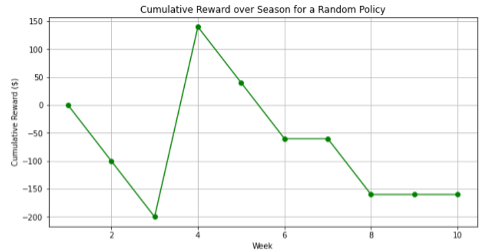
\includegraphics[width=0.7\textwidth]{season_reward.png}
    \caption{Random policy performance graph.}
\end{figure}


The initial approach will be to compare the betting odds to the difference in team Elo ratings--similar to power ratings--to determine if the risk is worth an expected reward. 
Additionally, we plan to incorporate offensive and defensive expectations, "explosiveness", and play success rates into the decision-making process. We aim to use reinforcement 
learning-based methods like Q-learning or Sarsa, to develop our optimal policies. Returning an optimal betting policy informed by a reward function of our determination is the end-goal of this project.

\begin{figure}[h!]
    \centering
    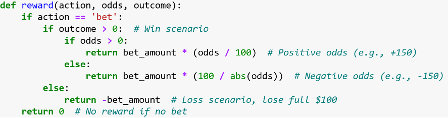
\includegraphics[width=0.7\textwidth]{reward.png}
    \caption{Reward performance across the season.}
\end{figure}

\section*{Deliverables}

The deliverables will include Profit vs. Time plots to compare the performance of different policies as they accumulate rewards throught a season. 
Initially, we will compare our model against a random policy to establish a baseline. Since only 11 weeks of betting data are available for seasons prior to 2024, we will rely on multiple sets of randomized  
policies and take the average to determine a baseline’s performance. Our goal is to show that our model consistently outperforms a random policy.


We will include as a future aspiration the extension the model to groupings of teams as such as conferences.  An extension such as this could explore expected reward of betting multiple games per week as opposed
to only on a single tema throughotu a season, though acquiring and formatting data for additional teams would prove challenging.

\section*{Questions for TA Feedback}
\begin{itemize}
    \item \textbf{Data sufficiency:} We are using only 11 weeks of data. Since the problem is sequential, the model will only have access to the outcome of the previous weeks of the season's data--causing the early 
    weeks of the season to rely on very small data sets, primarily sportsbook odds. Would it be beneficial to incorporate data from previous Stanford seasons to enrich the model’s learning process?
    \item \textbf{Method selection:} Are there any other methods that you would recommend for this type of problem? We’re considering Q-learning and Sarsa but are open to suggestions.
\end{itemize}

\section*{Conclusion}

We’re currently focused on developing reward function that can accurately reflect profitable betting strategies using available statistics. We aim to demonstrate that our model outperforms a random policy for the 2023 
Stanford football season and explore extending the model to other teams and betting websites as future work.

\end{document}